
\documentclass{book}
\usepackage{book}
\title{Jaseci and Jac}
\author{Jason Mars}


\newcommand{\printfigGraphTypes}{
    \begin{figure}
        \begin{subfigure}{.5\textwidth}
            \centering
            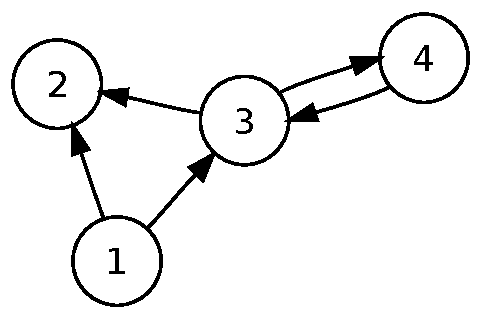
\includegraphics[width=.8\linewidth]{assets/images/Directed_graph_no_background.svg.pdf}
            \caption{Directed graph with cycle between nodes three and four.}
            \label{fig:directedgraph}
        \end{subfigure}
        \begin{subfigure}{.5\textwidth}
            \centering
            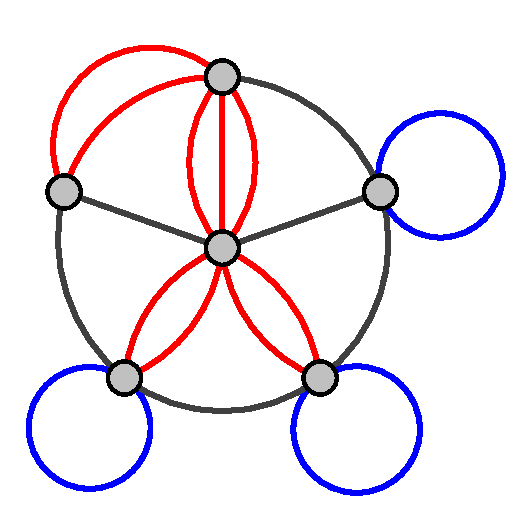
\includegraphics[width=.8\linewidth]{assets/images/Multi-pseudograph.svg.pdf}
            \caption{Multigraph with parallel edges and self-loops}
            \label{fig:multigraph}
        \end{subfigure}%
        \caption[]{Examples of first order graph symantics supported by Jaseci.\footnotemark}
        \label{fig:graph_examples}
    \end{figure}
    \footnotetext{Images credits to wiki contributers~\cite{wiki:Directed_graph_no_background.svg,wiki:Multi-pseudograph.svg}}
}


\newcommand{\printfigHelloWorldBaby}{
    \begin{figure}%{r}{0.5\textwidth}
        \centering
        
\includegraphics[width=.3\linewidth]{assets/images/hello_world_baby.jpg}
        \caption[]{World's youngest coder with valid HTML on shirt.\footnotemark}
        \label{fig:hello_baby}
    \end{figure}
    \footnotetext{Image credit to wiki contributer~\cite{wiki:hello_world_baby.jpg}}
}

\newcommand{\printtabPrecedence}{
    \begin{table}[t]
        \footnotesize
        \centering
        \begin{tabular}{l l l}
            \toprule
            \textbf{Rank} & \textbf{Symbol}                            & \textbf{Description}                           \\
            \midrule
            1             & \texttt{( ), [ ], ., ::, spawn}            & Parenthetical/grouping, node/edge manipulation \\
            2             & \texttt{\textasciicircum, []}              & Exponent,  Index                               \\
            3             & \texttt{*, /, \%  }                        & Multiplication, division, modulo               \\
            4             & \texttt{+, -}                              & Addition, subtraction                          \\
            5             & \texttt{==, !=, >=, <=, >, <, in, not in } & Comparison                                     \\
            6             & \texttt{\&\&, ||, and, or  }               & Logical                                        \\
            7             & \texttt{-->, <--, -[]->, <-[]-}            & Connect                                        \\
            8             & \texttt{=, +=, -=, *=, /=, := }            & Assignment                                     \\
            \bottomrule
        \end{tabular}
        \caption{Precedence of operations in Jac}
        \label{tab:jacprecedence} % Unique label used for referencing the table in-text
        %\addcontentsline{toc}{table}{Table \ref{tab:jacprecedence}} % Uncomment to add the table to the table of contents
    \end{table}
}

\newcommand{\printtabJSAPI}{
    \begin{table}[h]
        \footnotesize

        \begin{tabular}{l p{10cm}}
            \toprule
            \textbf{Interface}  & \textbf{Parameters}                                                                                                   \\
            \midrule
            check loggers       & ()                                                                                                                    \\
            config delete       & (name: str)                                                                                                           \\
            config exists       & (name: str)                                                                                                           \\
            config get          & (name: str)                                                                                                           \\
            config list         & ()                                                                                                                    \\
            config set          & (name: str, value: str, do\_check: bool = True)                                                                       \\
            alias clear         & ()                                                                                                                    \\
            alias delete        & (name: str)                                                                                                           \\
            alias list          & ()                                                                                                                    \\
            alias register      & (name: str, value: str)                                                                                               \\
            architype delete    & (arch: architype, snt: sentinel = None)                                                                               \\
            architype get       & (arch: architype, format: str = 'default', detailed: bool = False)                                                    \\
            architype list      & (snt: sentinel = None, detailed: bool = False)                                                                        \\
            architype register  & (snt: sentinel = None, code: str = `', encoded: bool = False)                                                         \\
            graph active get    & (detailed: bool = False)                                                                                              \\
            graph active set    & (gph: graph)                                                                                                          \\
            graph create        & (set\_active: bool = True)                                                                                            \\
            graph delete        & (gph: graph)                                                                                                          \\
            graph get           & (gph: graph = None, format: str = 'default', detailed: bool = False)                                                  \\
            graph list          & (detailed: bool = False)                                                                                              \\
            graph node get      & (nd: node, ctx: list = None)                                                                                          \\
            graph node set      & (nd: node, ctx: dict, snt: sentinel = None)                                                                           \\
            object get          & (obj: jaseci.element.element, detailed: bool = False)                                                                 \\
            sentinel active get & (detailed: bool = False)                                                                                              \\
            sentinel active set & (snt: sentinel)                                                                                                       \\
            sentinel delete     & (snt: sentinel)                                                                                                       \\
            sentinel get        & (snt: sentinel = None, format: str = 'default', detailed: bool = False)                                               \\
            sentinel list       & (detailed: bool = False)                                                                                              \\
            sentinel register   & (name: str, code: str = '', encoded: bool = False, auto\_run: str = 'init', ctx: dict = {}, set\_active: bool = True) \\
            walker delete       & (wlk: walker.walker, snt: sentinel = None)                                                                            \\
            walker execute      & (wlk: walker.walker)                                                                                                  \\
            walker get          & (wlk: walker.walker, format: str = 'default', detailed: bool = False)                                                 \\
            walker list         & (snt: sentinel = None, detailed: bool = False)                                                                        \\
            walker prime        & (wlk: walker.walker, nd: node = None, ctx: dict = {})                                                                 \\
            walker register     & (snt: sentinel = None, code: str = '', encoded: bool = False)                                                         \\
            walker run          & (name: str, nd: node = None, ctx: dict = {}, snt: sentinel = None)                                                    \\
            walker spawn        & (name: str, snt: sentinel = None)                                                                                     \\
            walker unspawn      & (wlk: walker.walker)                                                                                                  \\

            \bottomrule
        \end{tabular}
        \caption{Precedence of operations in Jac}
        \label{tab:jsAPI}
        %\addcontentsline{toc}{table}{Table \ref{tab:jacprecedence}} % Uncomment to add the table to the table of contents
    \end{table}
}
\newglossaryentry{christen}
{
    name=christen,
    description={to name or dedicate (something, such as a piece of code) by a ceremony that often involves breaking a bottle of champagne}
}
\newglossaryentry{scat}
{
    name=scat,
    description={the excrement of an animal including but not limited to human; also heroin }
}
\newglossaryentry{pwn}
{
    name=pwn,
    description={the act of dominating a person, place, or thing. (...or a piece of code)}
}
\newglossaryentry{gobbledygook}
{
    name=gobbledygook,
    description={language that is meaningless or is made unintelligible by excessive use of abstruse technical terms; nonsense}
}
\newglossaryentry{bleh}
{
    name=bleh,
    description={mildly yucky}
}
\newglossaryentry{leet}
{
    name=leet,
    description={v. hyper-sophisticated from a coding perspective, n. a language used by \gls{leet} \gls{haxor}s}
}

\newglossaryentry{haxor}
{
    name=haxor,
    description={\gls{leet} spelling of hacker}
}
\newglossaryentry{coder}
{
    name=coder,
    description={the superior human}
}
\newglossaryentry{Jaseci jolt}
{
    name=Jaseci jolt,
    description={an insight derived from Jaseci that serves as a high voltage bolt of energy to the mind of a sharp coder.}
}
\newglossaryentry{common languages}
{
    name=common languages,
    description={typical languages programmers use to write commercial software, (e.g., C, C++, Java, Javascript, Python, Ruby, Go, Perl, PHP, etc.)}
}

\newglossaryentry{grok}
{
    name=grok,
    description={to fully comprehend and understand deeply }
}

\newglossaryentry{sick}
{
    name=sick,
    description={\gls{redonkulous}}
}

\newglossaryentry{redonkulous}
{
    name=redonkulous,
    description={\gls{dope}}
}

\newglossaryentry{dope}
{
    name=dope,
    description={\gls{sick}}
}

\newglossaryentry{goo goo gaa gaa}
{
    name=goo goo gaa gaa,
    description={the language of babies}
}

\newglossaryentry{directed graphs}
{
    type=technical,
    name=directed graphs,
    description={}
}
\newglossaryentry{undirected graphs}
{
    type=technical,
    name=undirected graphs,
    description={}
}

\newglossaryentry{multigraphs}
{
    type=technical,
    name=multigraph,
    description={}
}

\newglossaryentry{hypergraphs}
{
    type=technical,
    name=hypergraph,
    description={}
}

\newglossaryentry{contexts}
{
    type=technical,
    name=contexts,
    description={A set of key value pairings that serve as a data payload attributable to nodes and edges in Jaseci graphs}
}

\newglossaryentry{walker}
{
    type=technical,
    name=walker,
    description={An abstraction in the Jaseci machine and Jac programming language that represents a computational agent that computes and travels along nodes and edges of a graph}
}

\begin{document}

% \chapter*{Copyright}
% \chapter*{Acknowledgments}
% \addcontentsline{toc}{chapter}{Acknowledgments}
% \chapter*{How To Send Feedback}

\cleardoublepage % Make toc appear on right side.
\setcounter{secnumdepth}{3} % toc is 2 level deep.
\tableofcontents
\pagebreak
\printglossary[title=Terms Used, toctitle=List of Terms]
\printglossary[type=technical, title=Technical Terms Used, toctitle=List of Technical Terms]


\chapter*{Preface}
\addcontentsline{toc}{chapter}{Preface}

The way we design and write software to do computation and AI today sucks. It's a vat of boiling poop, mixed with pee, slowly swirling and bubbling toward that dehydrated semi-solid state of goop that serves to repel and repulse most normal people only attracting the few unfortunate-fortunate folks that happen to be obsessed with \gls{scat}.
\par
Hrm, too much? Probably. I guess you'd expect me to use concrete examples and cite evidence to make my points, me being a professor and all. I mean, I could write something like \textit{``The fundamental imperative programming model utilized in near all of the production software produced in the last four decades has not changed since blah blah blah..."} to meet expections. I'd certainly sound more credible and perhaps super smart. Well, I'm not going to do that here. Let's have fun. Afterall, Jaseci has never been work for me, its play. Very ambitious play granted, but play at it's core.
\par
Everything here is based on my opinion and intution. That suffices for me, and I hope it does for you. I have spent many decades coding and leading teams who code, but its my gut that tells me that we can do better. This book describes my attempt at better. I hope you find value in it. If you do, awesome! If you don't, also awesome.


\chapter{Introduction}


\chapter{What and Why is Jaseci?}
\section{Viewing the Problem Landscape Spacially}
\section{Compute via The Collective, The Worker Bee Model}

\chapter{Abstrations of Jaseci}
\section{Graphs, the Friend that Never Gets Invited to the Party}
There's something quite strange that has happend with our \gls{common languages} over the years, ...decades. When you look at it, almost every data structure we programmers use to solve problems can be modeled formally as a graph, or a special case of a graph, (save perhaps hash tables). Think about it, stacks, lists, queues, trees, heaps, and yes, even graphs, can be modeled with graphs. But, low and behold, no common language ustilizes the formal semantics of a graph as its first order abstraction for data or memory. I mean, isn't it a bit odd that practically every data structure covered in the language-agnostic classic foundational work \textit{Introduction to Algorithms}~\cite{intro_to_algo} can most naturally be be reasoned about as a graph, yet none of the common languages have built in and be designed around this primitive. I submit that the graph semantic is stupidly rich, very nice for us humans to reason about, and, most importantly for the purpose of Jaseci, is inherently well suited for the conceptualization and reasoning about computational problems.
\par
There are a few arguments that may pop into mind at this point of my conjecture.
\begin{itemize}
    \item ``Well there are graph libraries in my favorite language that implement graph symantics, why would I need a language to force the concept upon me?''
          or
    \item ``Duh! Interacting with all data and memory through graphical abstractions will make the language ssllooowww as hell since memory in hardware is essitially a big array, what is this dude talking about!?!?''
\end{itemize}
\par
For the former of these two challenges, I counter with two points. First, the core design of a language are always based upon its inherent abstractions, and with graphs not being one such abstraction the language's design will not be optimized to empower programmers to nimbly do gymnastics with the rich symantics that graphs offer. And second, libraries suck (See~\ref{rant:librariessuck}).
\par
For the latter question, I'd respond, ``Have you SEEN the kind of abstractions in modern languages!?!? It's rediculous, lets look at python dictionaries, actually scratch that, lets keep it simple and look at dynamic typing in general. The runtime complexity to support dynamic typing is most certainly hgiher than what would be needed to support graph symantics. Duh right back at'ya!''
\subsection{Yes, But What Kind of Graphs}

There are many categories of graphs to consider when thinking about the abstractions to support in Jaseci. There are rules to be defined as to the availabe semantics of the graphs. Should all graphs be \gls{directed graphs}, should we allow the creation of \gls{undirected graphs}, what about parallel edges or \gls{multigraphs}, are those explicitly expressible or discouraged / banned, can we express \gls{hypergraphs}, and what combination of these graphical sematics should be able to be manifested and manipulated through the programming model. At this point I can feel your eyes getting droopy and your mind moving into that intermediary state between concious and sleeping, so let me cut to the answer.
\par
\printfigGraphTypes
In Jaseci, we elect to assume the following semantics:
\begin{enumerate}
    \item Graphs are directed (as per Figure~\ref{fig:directedgraph}) with a special case of a doubly directed edge type which can be utilized practically as an undirected edge (imagine fusing the two edges between nodes 3 and 4 in the figure).
    \item Both nodes and edges have their own distinct identities (i,e. an edge isn't representable as a pairing of two nodes). This point is important as both nodes and edges can have \gls{contexts}.
    \item Multigraphs (i.e., parallel edges) are allowed, including self-loop edges (as per Figure~\ref{fig:multigraph}).
    \item Graphs are not required to be acyclic.
    \item No hypergraphs, as I wouldn't want Jaseci programmers heads to explode.

\end{enumerate}
\emph{As an aside, I would describe Jaseci graphs as strictly unstrict directed multigraphs that leverages the semantics of parallel edges to create a laymans `undirected edge' by shorthanding two directed edges pointed in opposite directions between the same two nodes.}
\paragraph{[START NERD ALERT]}
\par
I'd formally describe a Jaseci Graph as an $7$-tuple $(N,E,C,s,t,c_N,c_E)$, where
\begin{enumerate}
    \item $N$ is the set of nodes in a graph
    \item $E$ is the set of edges in a graph
    \item $C$ is the set of all contexts
    \item $s$: $E \rightarrow V$, maps the source node to an edge
    \item $t$: $E \rightarrow V$,  maps the target node to an edge
    \item $c_N$: $N \rightarrow C$, maps nodes to contexts
    \item $c_E$: $E \rightarrow C$, maps edges to contexts
\end{enumerate}
An undriected edge can then be formed with a pair of edges $(x, y)$ if three conditions are met,
\begin{enumerate}
    \item $x, y \in E$
    \item $s(x) = t(y)$, and $s(y) = t(x)$
    \item $c_E(x) = c_E(y)$
\end{enumerate}
\paragraph{[END NERD ALERT]}
\par
If you happend to have read that formal definition and didn't enter deep comatose you may be wondering ``Whoa, what was that context stuff that came outta nowhere! What's this guy trying to do here, sneaking a new concept in as if it was already introduced and described.''
\par
Worry not friend, lets discuss.
\subsection{Putting it All Into Context}

A key principle of Jaseci is to reshape and reimagine how we view data and memory. We do so by fusing the concept of data wit the intuitive and rich semantics of graphs as the lowest level primitive to view memory.

A context is a representation of data that can be expressed simply as a $3$-tuple $(\sum_K,\sum_V,p_K)$, where
\begin{enumerate}
    \item $\sum_K$ is a finite alphabet of keys
    \item $\sum_V$ is a finite alphabet of values
    \item $p_K$ is the pairing of keys to values
\end{enumerate}

\section{Walkers}
\section{Abilities}
\section{Other Abstractions Not Yet Actualized}

\chapter{Architecture of Jaseci and Jac}
\section{Anatomy of a Jaseci Application}
\section{The Jaseci Machine}
\subsection{Machine Core}
\subsection{Jaseci Cloud Server}

\chapter{Interfacing a Jaseci Machine}
\section{JSCTL: The Jaseci Command Line Interface}
\section{Jaseci Rest API}

\chapter{The Jac Programming Language}


\chapter{Architecting Jaseci Core}


\chapter{Architecting Jaseci Cloud Serving}

\chapter*{Epilogue}
\addcontentsline{toc}{chapter}{Epilogue}

\appendix
\chapter{Rants}
\section{Why Libraries Suck}
\label{rant:librariessuck}
\par
Because they do.
\par
Still need more reasons?
\par
Well, if you dont already know, I'm not going to tell you.
\par
Fine, I'll tell you.
\begin{enumerate}
    \item They suck because they create dependancies for which you must have faith in the implementer of the library to maintain and keep bug free.
    \item They suck because there are often at least 10 options to choose from with near exact features expressings slightly different idosyncratic ways.
    \item They suck because they suck.
\end{enumerate}
Don't get me wrong, we have to use libraries. I'm not saying go reimplement the wheel 15 thousand times over. But that doesn't mean they don't suck and should be avoided if possible. The best is to know your library inside and out so the moment you hit some suckitude you can pull in the library's source code into your own codebase and \gls{pwn} it as your own.



\bibliographystyle{plain}
\bibliography{book}
\end{document}
